
\chapter{Conceptual Model for Reactive Information Systems and their Services}
% \\...Reactive Web Systems
% \\...Reactive Services
% \\...Web-based Event-Action Services}

% top down now, show whats beautiful and get everything together to get there



% Rahmenbedingungen
% Vorzuege
% Notwendigkeiten
% Architektur
% Schema: Zeit / Verteiltheit
%

% Steckbrief von Prototyp erstellen
 % was muss man ausfüllen um UC zu erstellen?
% why are we now suddenly responsive? we loosened up certain things

In the previous chapter we have shown that services in the Web and reactivity through programmability have received a great deal of attention.
Our goal is to combine both research fields in order to achieve reactivity within the Web by orchestrating its information space. 

\section{From Real Events to Events in the Web}
Real events are always bound to a spatial location and a point on the time axis.
An earthquake for example always has an epicenter and an occurence time.
Different points on earth's surface would feel the earthquake, which originates from the same epicentre, at a different point in time with a different intensity.
A Web event model of an earthquake would consist of a large number of identical \textrm{\textbf{ground-shake}} events that occur at different points in time and places.
Therefore they would hold different spatial location informations and intensities.
These events can be thought of as emmited into the Web by a seismometer sitting at the corresponding location.
\begin{figure}[!ht]
  \centering
  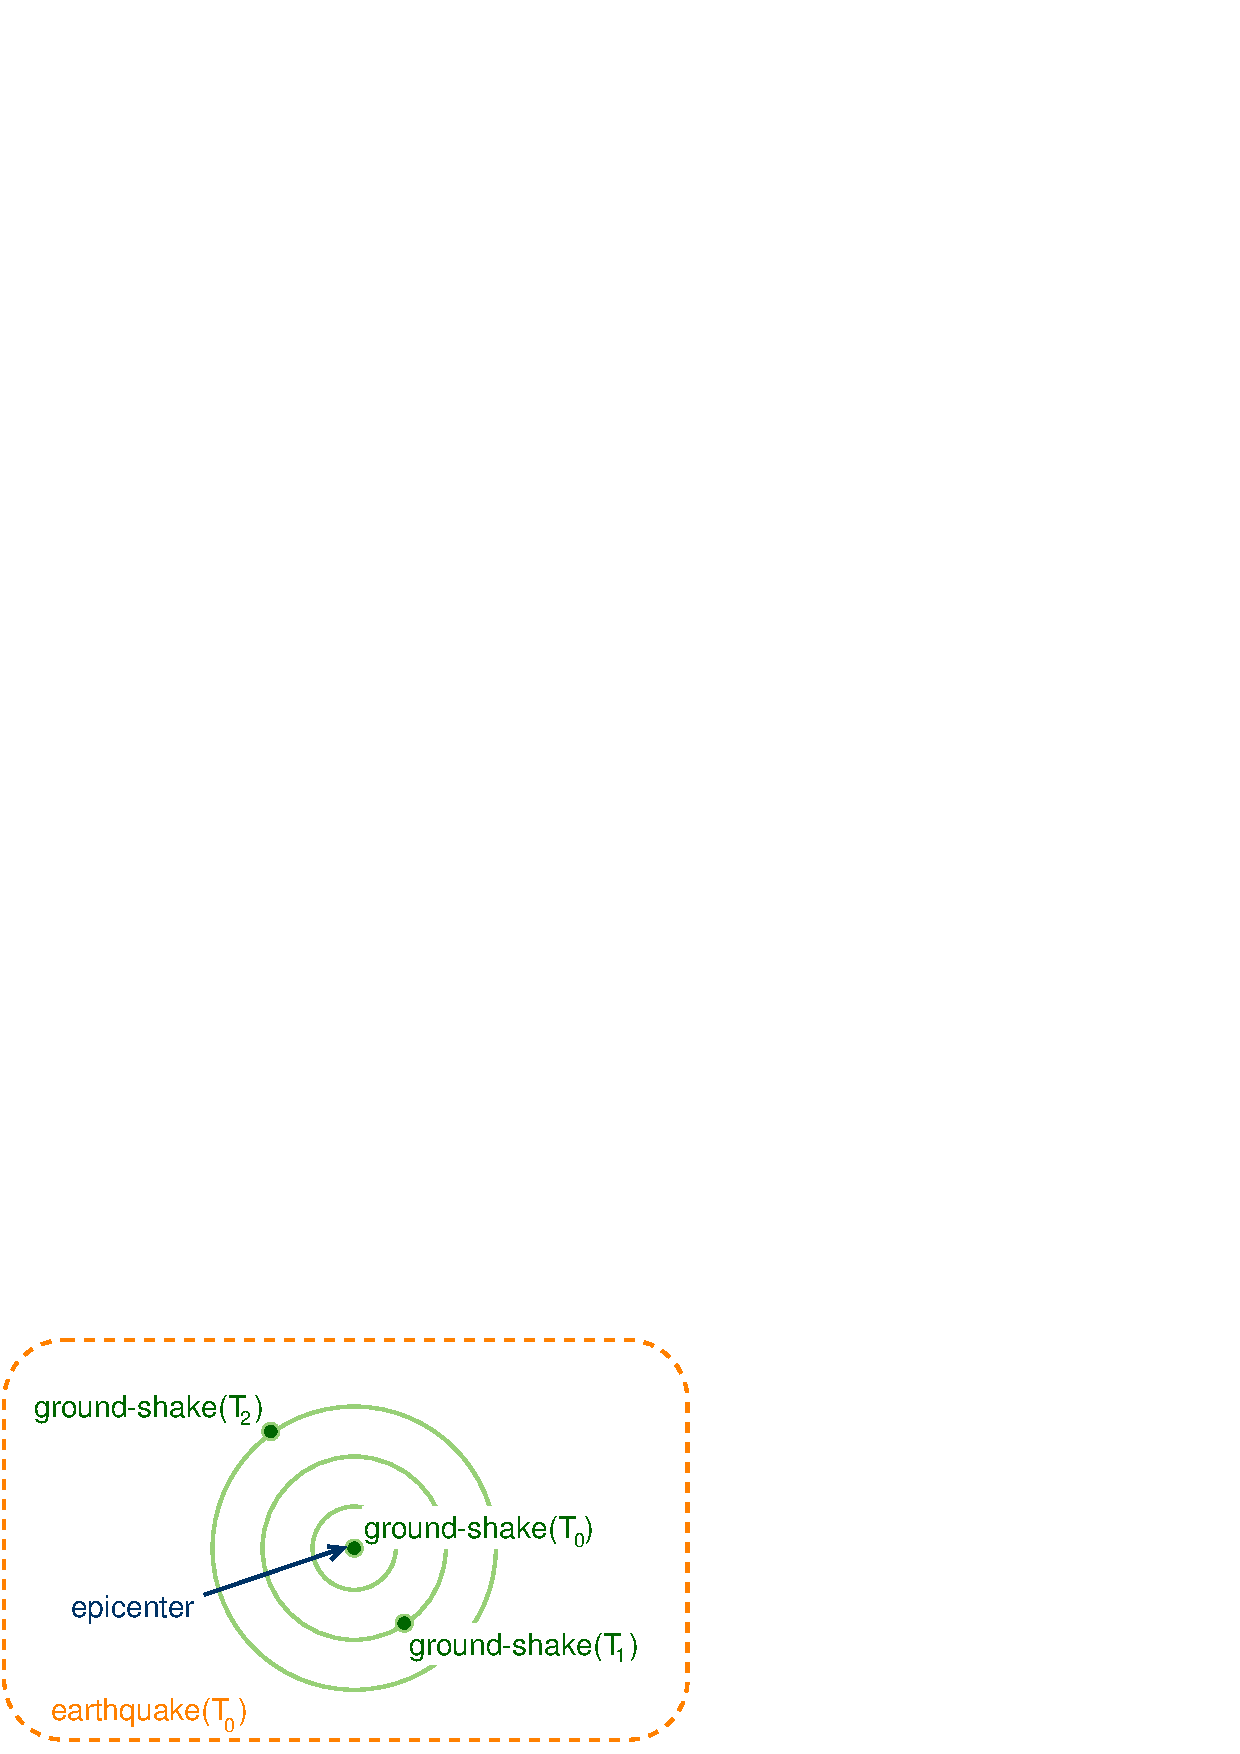
\includegraphics[width=0.6\textwidth]{figures/Earthquake}
  \caption{Web Event Model of an Earthquake}
  \label{fig:Earthquake}
\end{figure}

Within the Web, events lose their tight coupling to locations and retain only a time component.
The event instances keep this information as descriptive metadata.
A reactive system such as we envision it, could detect these \textrm{\textbf{ground-shake}} events and react on behalf of each one of them.
Because of the Web's latency these events do most certainly not arrive at systems within the Web in the original order, in which they were triggered.
They also do most likely not arrive in the exact same order for all systems.
This leaves us with time as the only important factor left, to distinguish events from each other in the first place.
To get an earthquake event out of all these ground shaking informations floating through the Web, somebody would need a reactive system that detects these events and assembles them into one earthquake event, together with a computed epicenter and magnitude.
Such a system (we call it \textrm{\textbf{earthquake-tracker}}) would own an earthquake model that allows it to decide wether a \textrm{\textbf{ground-shake}} event belongs to one physical earthquake or to another one, depending on its spatial location information and the intensity at that point in time.
It could then emit a more complex \textrm{\textbf{earthquake}} event (with epicenter and magnitude) that allows other systems to interpret this physical event and react on behalf of it.

Let's take another system that reacts on a physical earthquake.
It is now left with a multitude of different options on how to react.
It could only react on the \textrm{\textbf{earthquake}} event which is coming from the system above (\textrm{\textbf{earthquake-tracker}}) that applies its earthquake model to the incoming \textrm{\textbf{ground-shake}} events.
But how long will it take for this system to deploy its \textrm{\textbf{earthquake}} event?
Eventually it waits for one round-trip of a seismic wave around the world, which takes approximately half an hour.
What if it waits two or three round-trip times in order to collect more accurate data?
And what if our new system wants to react as fast as possible in order to warn people all around the world.
It would then need to react on a small subset of the \textrm{\textbf{ground-shake}} events in order to quickly identify a real earthquake and take measurements, e.g. immediately send out text messages to people, or to deploy yet another ( this time \textrm{\textbf{earthquake-alert}}) event into the Web's information space.
This relatively simple example discloses the complex nature of event-driven systems, but also their high flexibility and fine grained tuning possibilities.

\section{The Web's Event \& Action Information Space}
\index{Information Space}
For a conceptual model, the information space in which the events are triggered and the actions are invoked, needs to be identified.
During our research we encountered many different event or action providing subsets of the Web that can be incorporated into our model:
\begin{itemize}
  \item \textrm{World-Wide Web}
  \item \textrm{Services in the Web}
  \item \textrm{Web of Things}
\end{itemize}
We have already shown in chapter "Related Work", that there are basically two different ways how the Web's information space is accessible, i.e. either functionality and data have to be requested, or data is pushed through Webhooks.
All of the above listed information space subsets require at least one of these two access methodologies.
And through these access methodoligies are we able to turn the information space of the Web into events and actions.
\index{World-Wide Web}
The \textrm{World-Wide Web}~\cite{DBLP:journals/en/Berners-LeeCGP92}, as envisioned by Tim Berners-Lee, is an information universe of interlinked documents, that a user can browse through.
In our model, we can pull events directly from the World-Wide Web.
For example, most documents in the World-Wide Web are subject to changes and such changes can be translated into events.

\index{Services}
We gave an introduction into \textrm{Services in the Web} in chapter "Related Work"

\index{Web of Things}

Either there is an event producer which proactively pushes events into the Web, or a service is offered whose responses can be turned into events.
These events and actions can have a solely virtual nature or, in the case of data from the \textrm{"Web of Things"}, also a physical nature.
A virtual nature can be anything from a static webpage to offered services, such as a detected change on a webpage can become an event as well as a service answer is interpreted as such for example a new mail arriving.
A virtual action could be a babelibu.
A physical nature for events could for example be measurements from a rain detector, an action could be a window shutting automatically.

\begin{figure}[!ht]
  \centering
  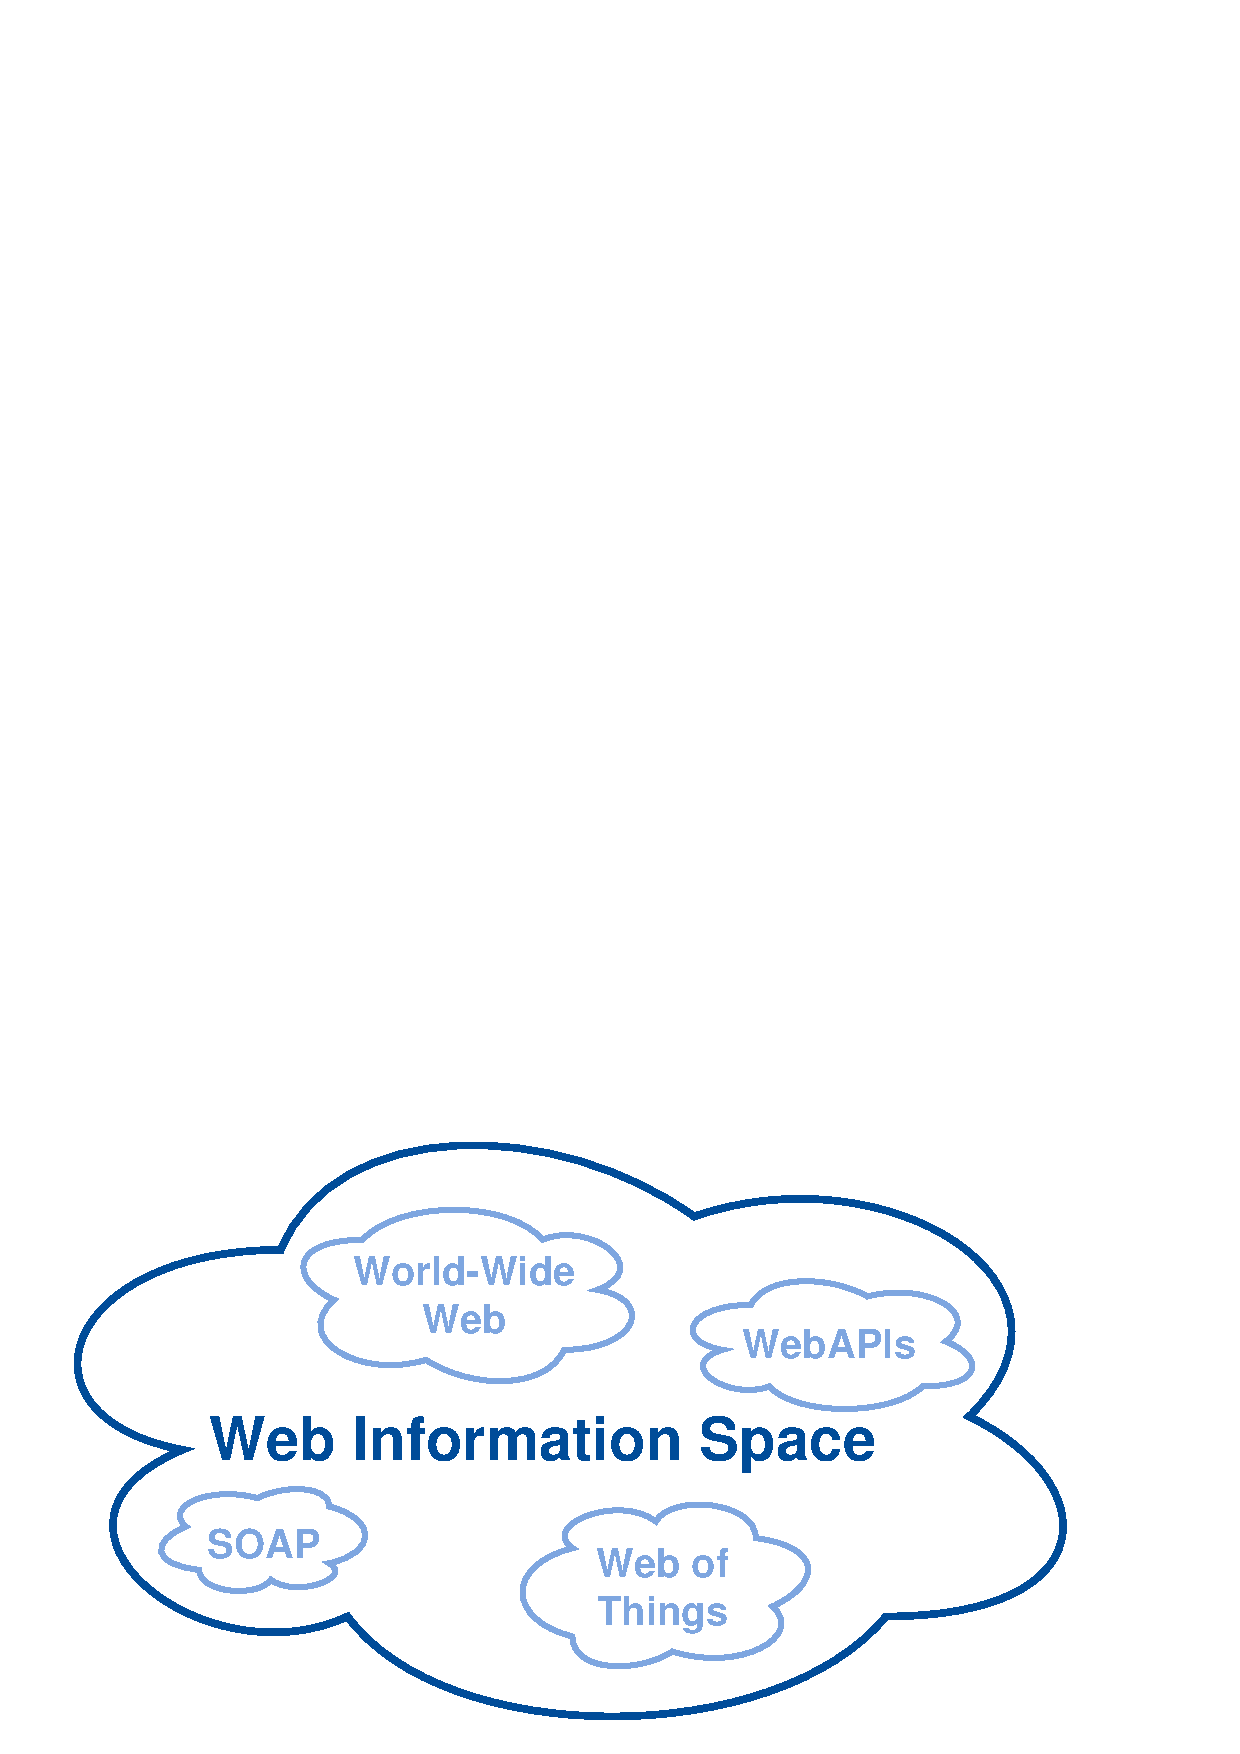
\includegraphics[width=0.6\textwidth]{figures/InformationSpace}
  \caption{The Web's Information Space}
  \label{fig:InformationSpace}
\end{figure}
There are different categories of events and also different ways how they can get into the Web:

We have seen in the related work chapter that there is a growing number of Web APIs which become accessible.


There are differrent categories in which we could 

% TODO Classify events in information space, information events: temperature, new mail, blabliblu
% TODO Classify Actions in information space
Actions
\begin{itemize}
  \item Event Redirection
  \item Event Amplification
  \item WebApp Actions
\end{itemize}


\section{Impose Reactivity in the Web Information Space}
% \subsection{Engine \& Rules}
% TODO conditions with examples
% Model / Schema
% Zeit / Verteiltheit

% RL <-> ECA
% TODO figure: ECA Schema
% TODO Figure: ECA in the distributed environemnt
% TODO figure: Rules (unions / objects / Rueckkoppelungen )

% \section{Event Condition Action (ECA) Model in the Web}
In the last section we showed how mashups create additional value for the Web by combining several WebAPI's.
But it turned out, that such mashups are closed systems, which ofen only allow little degree of parametrization.
To get past such limitations and define a conceptual model for reactive Web systems, it is necessary to define a 

existing rule languages, rule engines, 

Existing ECA systems all act on local data.
% (List examples) 
Looking at (Wikipedia...) their definition is actions on local data.
This does only add reactivity to these systems and not to the Web per se.

Such systems are merely event sinks which add fairly any value to the Web, except for the individual users and the system itself.

\begin{figure}[!ht]
  \centering
  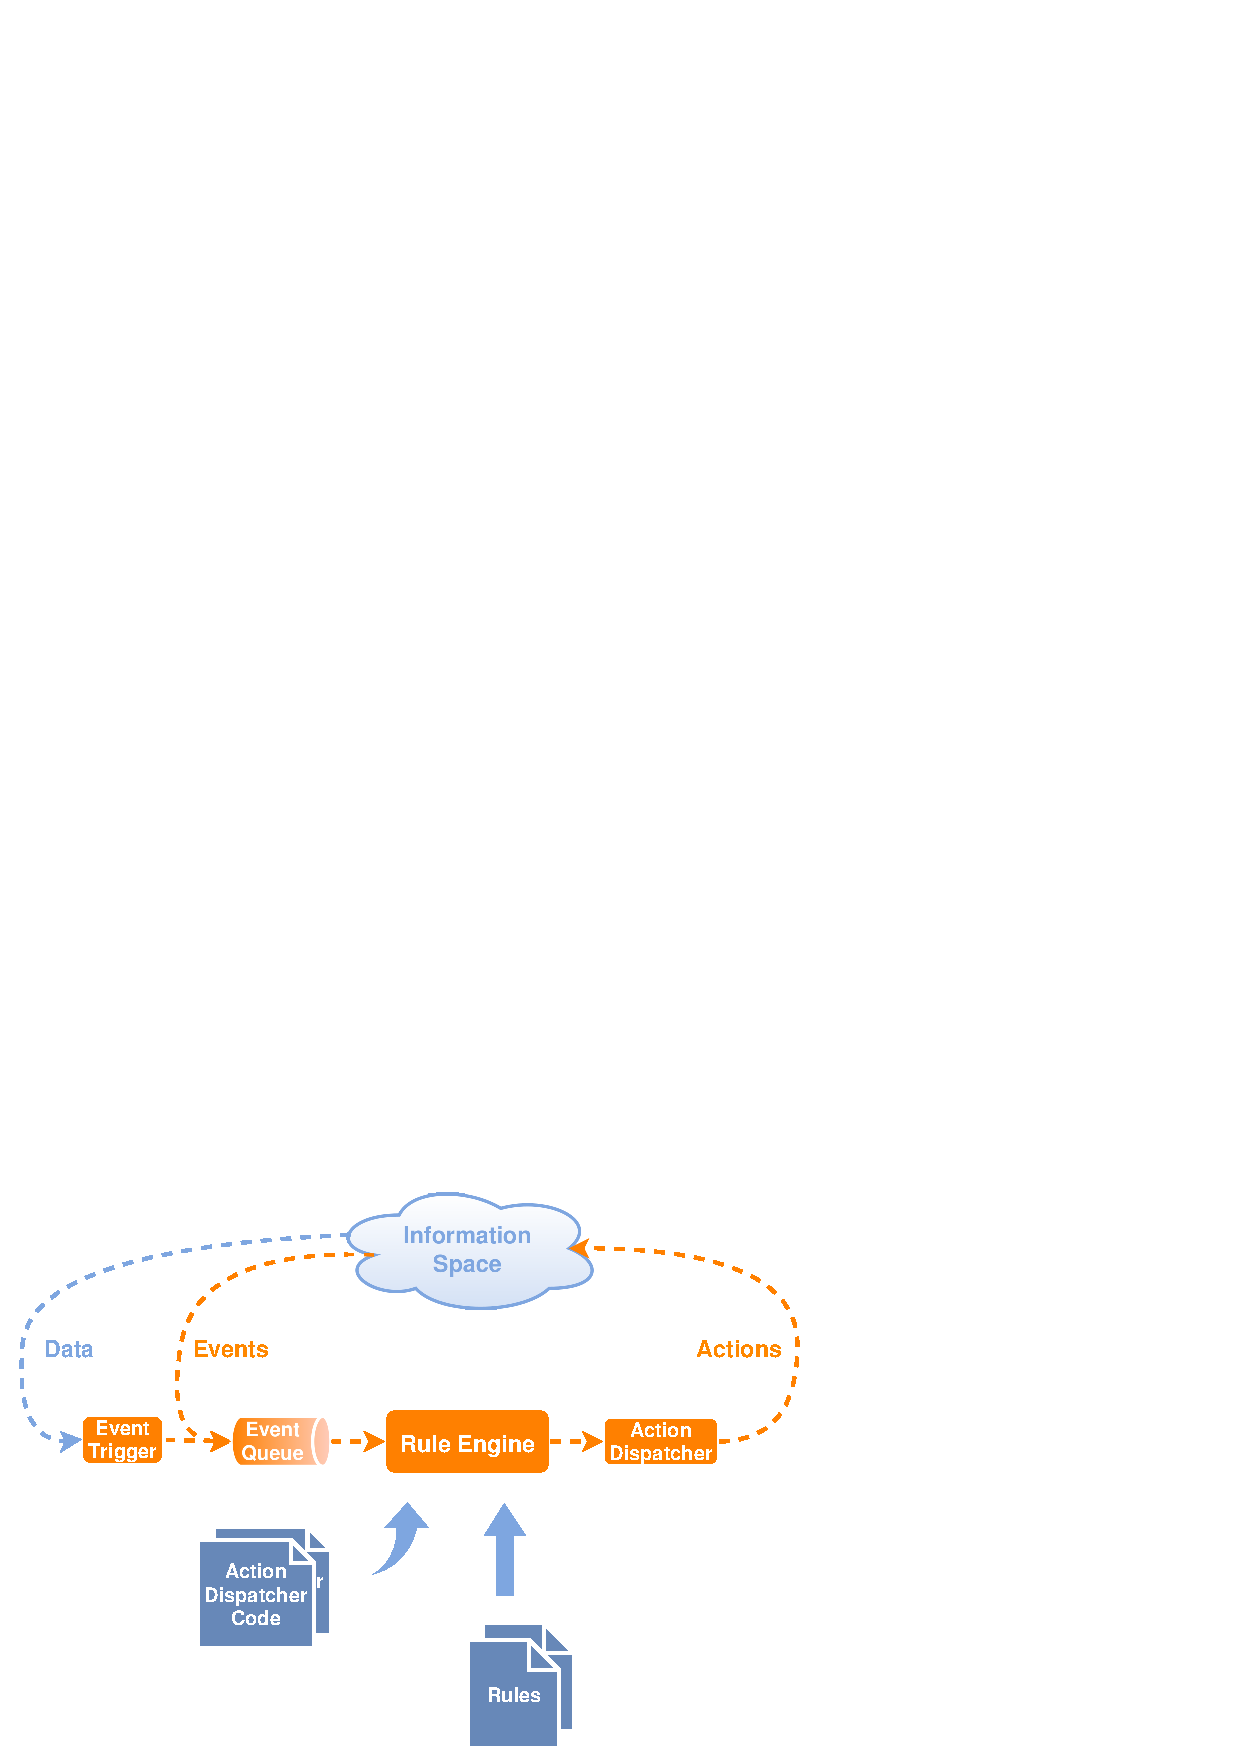
\includegraphics{figures/Standard-Model-Template}
  \caption{Conceptual Model for Reactive Information Systems}
  \label{fig:Standard-Model-Template}
\end{figure}


\begin{itemize}
  \item from Web to events
  \item from events to rules
  \item from rules to actions
  \item from actions to the Web
  \item from concept to engine
\end{itemize}


% Regelimplementierungssprache
\subsection{Conceptual Rule Language}
Describe conceptual rule language
ON (existing categories)
IF (condition boundaries)
DO (call to existing action modules with parameters)

a lot possible, but dangerous.

\begin{Verbatim}[fontsize=\small,commandchars=\\\{\}]
\PY{k}{on} \PY{n}{mail}
\PY{k}{if} \PY{n}{sender}\PY{o}{=}\PY{l+s+ss}{\PYZdq{}sender@mail.com\PYZdq{}}
\PY{k}{do} \PY{n}{webapi}\PY{o}{\PYZhy{}}\PY{o}{\PYZgt{}}\PY{l+s+s2}{newcontent}\PY{p}{(}\PY{n}{subject}\PY{p}{)}
\end{Verbatim}
